\documentclass[10pt]{article}
%\usepackage{geometry} % see geometry.pdf on how to lay out the page. There's lots.
\usepackage[left=3cm,top=3cm,right=3cm,bottom=3cm]{geometry}
\geometry{letterpaper} % or letter or a5paper or ... etc

\usepackage{graphicx}
\usepackage{amssymb}
\usepackage{epstopdf}
\usepackage{wrapfig}
\usepackage{float}
\usepackage[usenames,dvipsnames]{color}
\usepackage{mcode}
%\usepackage[authoryear, round, sort]{natbib}
\usepackage{color}
\usepackage{hyperref}
\hypersetup{colorlinks=true,linkcolor=black,anchorcolor=black,citecolor=MidnightBlue,filecolor=red,pagecolor=red,urlcolor= blue}
%\usepackage{citesupernumber}
%\usepackage{nature}
%\usepackage{naturefem}


\DeclareGraphicsRule{.tif}{png}{.pdf}{`convert #1 `dirname #1`/`basename #1 .tif`.pdf}
%\usepackage{fancyhdr}
%\pagestyle{fancy}
%\lhead{Effect of slow-wave activity on cortical processing }\chead{Project Proposal}\rhead{Dimitri Yatsenko}
%\rfoot{\today}
\usepackage[small,compact]{titlesec}
\setlength{\parskip}{6pt plus3pt}
\titlespacing{\section}{0pt}{*0}{*0}
\titlespacing{\subsection}{0pt}{*0}{*0}
\titlespacing{\subsubsection}{0pt}{*0}{*0}
\setlength{\parindent}{0.0cm}
\usepackage[small]{caption}
\usepackage{fourier} % math & rm

\title{DataJoint Tutorial}
\date{\today} % delete this line to display the current date
\author{Dimitri Yatsenko, Alexander Ecker, Andreas S. Tolias}

\begin{document}
\maketitle
\tableofcontents
\newpage
\section{Overview}
\subsection{What is DataJoint}
DataJoint is a MATLAB tool for the distributed processing and management of large volumes of data in a science lab.  DataJoint is built on the foundation of the \href{http://en.wikipedia.org/wiki/Relational_model}{relational data model} and prescribes a consistent method for organizing, populating, and querying the data with minimal chance of loss of data integrity.

\subsection{History}
DataJoint was developed by Dimitri Yatsenko in Andreas Tolias' lab at Baylor College of Medicine beginning in October 2009 with the first alpha release scheduled for March 2011. DataJoint was inspired in part by the earlier data management tool in the lab called Steinbruch developed by Alex Ecker and Philipp Berens.

\subsection{Prerequisites}
We assume that the reader is proficient with MATLAB and its object-oriented features in particular.  Readers do not need to be a priori familiar with relational databases but will need to master the basic relational concepts presented in this tutorial. We also assume the availability of a MySQL server in the lab with accounts and schemas for each user. The installation and administration of the MySQL server is not covered in this tutorial.

\subsection{Foundations}
DataJoint adheres faithfully to the theoretical rigor and simplicity of the relational model\footnote{See C.~Date, {\em SQL and Relational Theory}, 1$^{\textrm{st}}$ Edition, O'Reilly, 2009.}. This discipline then allows avoiding common pitfalls of data organization and affords simpler ways of querying data from multiple tables.   DataJoint's relational operators are \href{http://en.wikipedia.org/wiki/Algebraic_closure}{algebraically closed}, which means that their outputs can be assigned to variables and be used as operands in the next expression. As the result, even skilled SQL programmers may prefer formulating precise queries in DataJoint to composing analogous SQL code while novice users will quickly become proficient and efficient with a minimal set of correct relational concepts bypassing SQL's arcane syntax.

DataJoint relies on MySQL's native constructs for data organization.  All data organized in DataJoint is transparently accessible by other database interfaces.

\subsection{Components}
The current version of DataJoint is developed in MATLAB 2007. For its database interface, DataJoint uses a modified version of the  \mcode{mym} library from \url{http://mym.sourceforge.net/}.

DataJoint comprises two MATLAB classes: \mcode{DeclareDJ} and \mcode{DJ}.  

\mcode{DeclareDJ} is used for data definition. It creates tables and sets their dependencies under a set of conventions that encourage a solid relational data model. 

\mcode{DJ} implements all data query and manipulation functionality. Each table in a DataJoint schema has a homonymous class inheriting its functionality from \mcode{DJ}. \mcode{DJ} supports a relationally complete algebra that affords flexible, expressive, and succinct data queries.

\section{The relational data model}
\subsection{Background}
Invented by IBM researcher \href{http://en.wikipedia.org/wiki/Edgar_F._Codd}{Edgar F.~Codd} in 1969,\footnote{E.~F.~Codd. A relational model of data for large shared data banks. {\em Communications of the ACM}, 13(6):387, 1970} the \href{http://en.wikipedia.org/wiki/Relational_model}{relational model} for databases steadily replaced the earlier hierarchical and network models and has become the de facto standard for mainstream databases today, supporting banking transactions, airfare bookings, and data-intensive websites such as Facebook, Google, Wikipedia, and YouTube, to pick but a few examples.  Modern relational database management systems  execute fast, precise, and flexible data queries and preclude inconsistencies arising from simultaneous or interrupted manipulations by multiple users. Interactions with a relational database are performed in a query language such as \href{http://en.wikipedia.org/wiki/SQL}{SQL}. 

Below we provide a brief semiformal overview of basic concepts of relational concepts as implemented by DataJoint.  

\subsection{Attributes and tuples}
A {\em tuple} is a set of attribute name/value pairs. For example, the tuple
\begin{verbatim}
 mouse_id   measure_date   weight 
   1001      2010-10-10     21.5
\end{verbatim}

in a given relation may represent a real-world fact such as ``On Oct.~10, 2010, mouse \#1001 weighed 21.5 grams.''  An attribute name is more than just a name: it implies a particular {\em datatype} and a unique {\em role} in the tuple and in the external world.  Thus attribute names must be unique in a tuple and their order in the tuple is not significant.  

The closest equivalent of a tuple in Matlab is a structure. Therefore, we will use the terms {\em attribute} and {\em field} interchangeably.


\subsection{Relations}
A relation is a set of tuples that all have the same set of attribute names. No duplicate tuples can exist in a relation.  The ordering of tuples in a relation is not significant.  

Starting with {\em base relations} corresponding to {\em tables} in the database, we can transform them into {\em derived relations} by applying {\em relational operators} until they contain only all the necessary information, and then retrieve their values into the MATLAB workspace.  We will use the term {\em table} and {\em base relation} interchangeably. 

\subsection{Matching tuples}\label{sec:matching}
The key concept at the foundation of data manipulations in the relational model is {\em tuple matching}.  Two tuples match if their identically named attributes contain equal values.  Here are some examples: Two tuples may be merged into one if they match but not otherwise.  One tuple may be used to address other matching tuples in a relation.  The {\em join} (see \autoref{sec:join}) of two relations is the set of all matching pairs from the two relations, merged.

\subsection{Primary key}
In DataJoint, each relation must have a {\em primary key}, i.e.~a subset of its attributes that are designated to uniquely identify any tuple in the relation. No two tuples in the same relation can have the same combination of values in their primary key fields.  To uniquely identify a tuple in the relation, one must provide the values of the primary key fields as a matching tuple. 

\section{Data management in a science lab}
\subsection{Project schema}
In DataJoint, every study comprising a set of experiments and related data is organized as a dedicated schema: a collection of logically related tables (\autoref{fig:categories}).  DataJoint creates tables with properly configured referential integrity constraints and a dedicated MATLAB class that supports all manipulations on the table.

\begin{figure}[htb]
\center
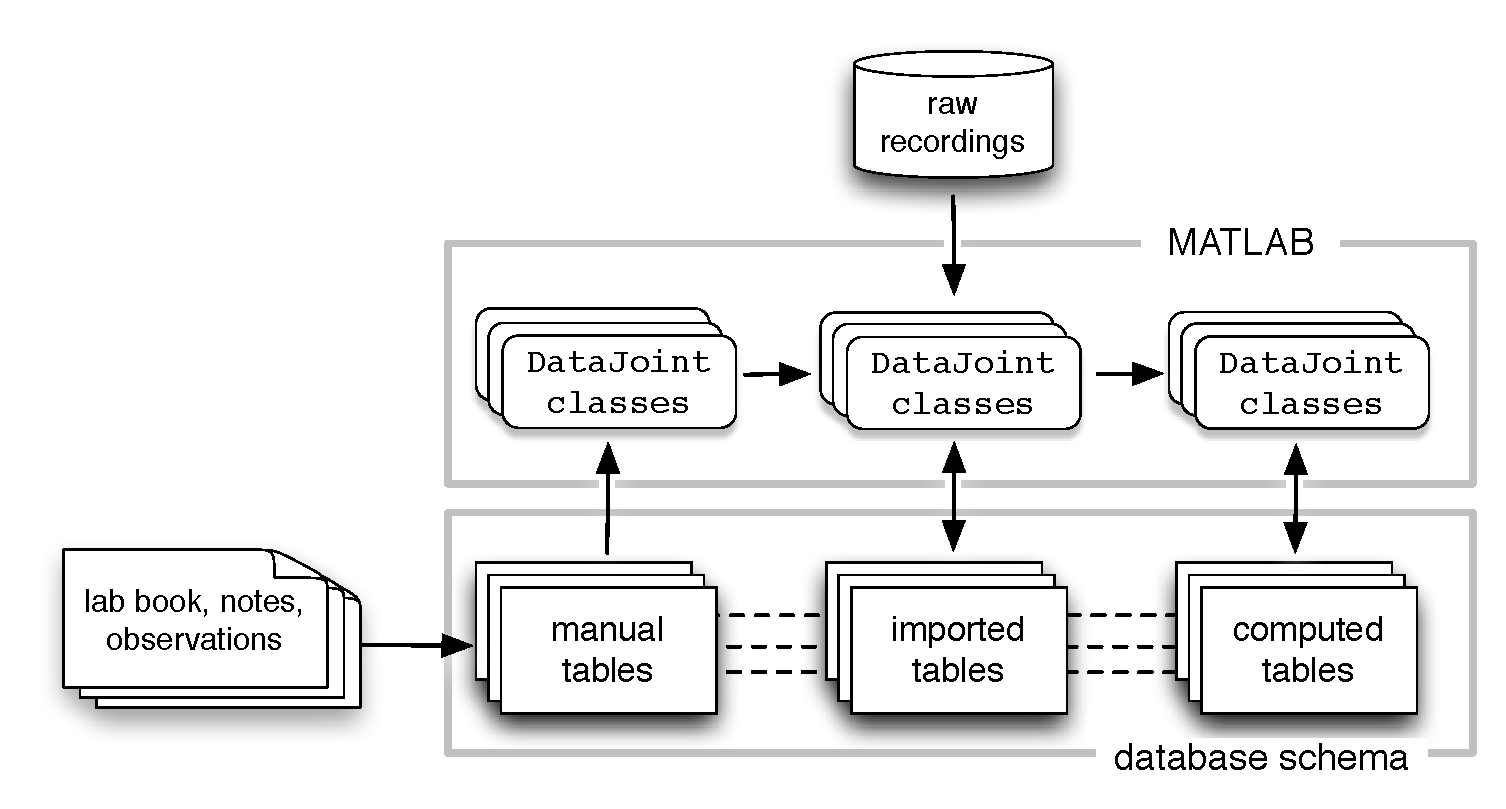
\includegraphics[width=0.75\textwidth]{categories.pdf}
\caption{Data organization in a DataJoint schema.}
\label{fig:categories}
\end{figure} 
 
\subsection{Data tiers}\label{sec:tiers}
Every table in a DataJoint schema is assigned one of the four tiers: {\em lookup tables}, {\em manual}, {\em imported}, and {\em computed}  (\autoref{fig:categories}):
\begin{enumerate}
   \item{\bf Lookup tables} contain information that is involved in setting up the processing chain itself: filter settings, algorithm parameters, etc.  Lookup tables are populated manually.
   \item{\bf Manual tables} contain information about experiments that is entered manually, e.g. subject information, independent variables, acquisition settings, visual observations, and paths to recorded data.  Due to their high value and small size, manual tables are backed up most frequently (e.g.~at every update).
   \item{\bf Imported tables} contain information extracted from  files outside the database (e.g.~raw recordings).  Raw recordings are typically in large files that cannot be kept online indefinitely. Once the extraction algorithms have stabilized and the extracted  data have been imported into the database, the raw recordings may be taken offline.  Imported tables are populated automatically and need to be backed up regularly, especially after the raw data files have been taken offline. 
   \item {\bf Computed tables} are populated automatically with data computed from other data already present in the database.  Data from computed tables are deleted automatically when their parent data are deleted. Computed tables do not typically need to be backed up at all.
\end{enumerate}  


\subsection{Illustration schema}
To illustrate DataJoint usage in practice, we provide a snippet of an actual schema used in our lab in \autoref{sec:vis2p}.


\section{Defining tables}\label{sec:definition}

This section explains how to create a set of interdependent tables with referential constraints using the class \mcode{DeclareDJ}.

\subsection{Configure the MySQL schema}
First, have the database administrator create a dedicated schema for your project.  You will receive the host name, username, password, and the schema name.

\subsection{Define the schema class}

For every schema, there must exist an abstract class which assigns the connection parameters and inherits from \mcode{DJ} all the relational methods.  All other will inherit from the schema class and will know how to connect to the database.  

The following code is the constructor for schema class \mcode{Vis2p}, which retrieves schema connection information from the global variable defined in the startup script. 

\begin{lstlisting}
function obj = Vis2p( tableName, varargin )
conn.host = '<host-address>';
conn.schema = '<your_project_schema>';
conn.user = '<user_name>';
conn.pass = '<password>';
conn.table  = '';
conn.schemaClass = mfilename;
if nargin>0
    assert( nargin>=1 && ischar(tableName), 'Invalid table or view name' );
    conn.table = tableName;
end
obj = class(struct,'Vis2p',DJ(conn,varargin{:})); 
\end{lstlisting}

In practice the connection parameters may be stored in a global variable that is set at startup to allow logging with different user credentials and into different schema while using the same code.  The schema name does not need to match the schema class name.

\subsection{Declare an independent table} 
Various types of discrete facts about your study must be assigned their own tables in the database. Let's begin with the manually populated table \mcode{Mice} that contains information about mice.  Begin the table declaration by instantiating a \mcode{DeclareDJ} object provided the schema class, the table name, and the table tier ({\em manual}, {\em lookup}, {\em imported}, or {\em computed} as described \autoref{sec:tiers}).

\begin{lstlisting}
ddj=DeclareDJ( Vis2p, 'Mice','manual' );
\end{lstlisting}

\subsection{Specify the primary key}  Each table must have one primary key: one field or a combination of fields that uniquely identify a row in the table.  The database uses the primary key to prevent duplicate entries, to relate data across tables, and to accelerate data queries. The choice of the primary key will determine how you identify data elements. Therefore, make the primary key {\bf short}, {\bf expressive}, and {\bf persistent}. Integers, dates, and timestamps make best primary key fields. To protect users from choosing poor primary key fields, DataJoint prohibits character strings, enums, and blobs from primary keys.

For example, mice in our lab are assigned unique IDs. The mouse ID can serve as the primary key for the table \mcode{mice}.  Add the field \mcode{mouse_id} to the table declaration:

\begin{lstlisting}
ddj=addKeyField(ddj,'mouse_id','smallint unsigned','unique mouse id (0-65535)');
\end{lstlisting}

A primary key comprising real-world attributes is called a \href{http://en.wikipedia.org/wiki/Natural_key}{natural primary key}.  If no convenient natural key already exists, you may choose to introduce a \href{http://en.wikipedia.org/wiki/Surrogate_key}{surrogate primary key}, i.e.~an artificial attribute whose purpose is to uniquely identify data elements.  For example, to identify American workers for taxation purposes, the U.S.~government assigns every worker a surrogate attribute, the social security number, but the government must go to great lengths to ensure that this primary key is assigned exactly once by checking against another less convenient candidate key (the combination of name, parents' names, date and place of birth, etc.)  As exemplified by the SSN, well managed surrogate keys tend to get institutionalized and become natural.  

\subsection{Add non-key table fields}
Now use the \mcode{addField} method to add fields by specifying their name (always lowercase), datatype, brief description, and (optional) default value:

\begin{lstlisting}
ddj=addField(ddj,'mouse_strain','enum("C57BL6/J","agouti")','');
ddj=addField(ddj,'mouse_dob','date','mouse date of birth');
ddj=addField(ddj,'mouse_sex','enum("F","M","unknown")','');
ddj=addField(ddj,'mouse_notes','varchar(1023)','free-text info about the mouse','');
\end{lstlisting}

Remember that field names (attribute name) must be sufficiently descriptive to identify their role in the relation and their domain.  Identically named fields in different relations are assumed to signify the same thing and can be used to match or join tuples across relations.  Make sure that fields only have identical names if they refer to the same attribute even in different tables.  For example, if both the  \mcode{Sessions} and \mcode{Scans} tables have a comment field, give them different names, e.g.~\mcode{sess_comment} and \mcode{scan_comment}.

The following datatypes are supported by DataJoint:
\begin{description}
\item[enum] one of several explicitly enumerated values specified as strings. Use this datatype instead of text strings to avoid spelling variations and to save storage space.  For example, for anesthesia, the datatype could be \mcode{enum} with values \mcode{"urethane"} and \mcode{"isoflurane"}.  Do not use enums in primary keys if you plan to change the enum values in the future.
\item[date] date as \mcode{'YYYY-MM-DD'}.
\item[timestamp]  Date and time to the second.  Also can be configured to timestamp data entries automatically.
\item[char]  a text string of specified length. Rarely used.
\item[varchar]  a text string of arbitrary length up to maximum length. Specify the max length. 
\item[decimal]  a number with a fixed number of fractional digits.  This is helpful to represent numbers whose magnitude is well defined and does not warrant the use of floating-point representation.  Specify the total number of decimal digits and the number of fractional digits.  Check \mcode{unsigned} if the values can only be nonnegative.
\item[float]  a single precision floating-point number.  Takes 4 bytes.  Single precision is sufficient for many measurements.
\item[double]  a double precision floating-point number. Takes 8 bytes.  
\item[int] a 32-bit integer number, ranging from -2,147,483,648 to 2,147,483,647.  Check \mcode{unsigned} to limit to nonnegative values, in which case the range is from 0 to 4,294,967,295.
\item[smallint] a 16-bit integer number, ranging from -32,768 to 32,767.  Check \mcode{unsigned} to limit to nonnegative values, in which case the range is from 0 to 65,535.
\item[tinyint] an 8-bit integer number, ranging from -128 to 127.   Check \mcode{unsigned} to limit to nonnegative values, in which chase the range is from 0 to 255.
\item[longblob] for MATLAB matrices, images, structures, and objects, up to 4 \href{http://en.wikipedia.org/wiki/Gibibyte}{GiB} in size.  DataJoint also allows smaller blobs 
{\bf mediumblob}, {\bf blob}, and {\bf tinyblob} to store up to 16 MiB, 64 KiB, and 256 B, respectively. 
\end{description}

Use the smallest most restrictive datatype sufficient for your data.  

If the field value is allowed to be missing from the table, specify the default value as \mcode{[]}. Missing field values will retrieved as empty cell arrays, empty strings, or NaNs, depending on the data type.

\subsection{Execute the declaration}
Now use the \mcode{execute} method to actually create the table in the database and automatically generate the template for its class. From your work directory, execute the table declaration:
\begin{lstlisting}
  dj = execute( ddj );
\end{lstlisting}

This command will create the class \mcode{Mice} in the current directory (unless it already existed elsewhere on the path) and its associated table in the database. 

It is safe to execute \mcode{DeclareDJ} multiple times without the risk of overwriting existing data. To modify an existing table, drop the previous table first, e.g.:
\begin{lstlisting}
   drop( Mice );  % drop table Mice from the database
\end{lstlisting}

You may add a comment describing the table:
\begin{lstlisting}
   setTableComment( Mice, 'Mouse information' );
\end{lstlisting}

The class \mcode{Mice} does not contain any information pertaining to the structure and contents of the table and retrieves it from the database at instantiation.  Its \mcode{display} method (or simply omitting the trailing semicolon) will display the structure of the table and its dependencies:

\begin{lstlisting}
>> Mice
\end{lstlisting}
\begin{scriptsize}
\begin{verbatim}
@Mice - a manual table   "Mouse information"
             - ATTRIBUTES -
           *mouse_id ::  smallint unsigned :: unique mouse id (0-65535).
        mouse_strain :: enum('C57BL6/J','a :: 
           mouse_dob ::               date :: mouse date of birth
           mouse_sex :: enum('F','M','unkn :: 
         mouse_notes ::      varchar(1023) :: free-text info about the mouse
             mice_ts ::          timestamp :: automatic timestamp.  Do not edit
         
         0 tuples
\end{verbatim}
\end{scriptsize}


Note that the primary key fields are marked with an asterisk. Also note that \mcode{DeclareDJ} added the automatic  timestamp field, which will contain the time at which each row in the table was last inserted (see also method \mcode{DeclareDJ/omitTimestamp}).

\subsection{Declare a dependent table}
Now let's use \mcode{DeclareDJ} to declare the manual table \mcode{Sessions}, which describes imaging sessions performed on mice.  A session cannot exist until the mouse exists and the database will maintain this constraint if \mcode{Mice} is declared as the parent of \mcode{Sessions}:

Displaying the new class \mcode{Sessions} will yield:
\begin{scriptsize}
\begin{verbatim}
@Sessions - a manual table   "Recording sessions"
     PARENT TABLES: @Mice
             - ATTRIBUTES -
           *mouse_id ::  smallint unsigned :: 
            *sessnum ::   tinyint unsigned :: imaging session number for this mouse
           sess_date ::               date :: imaging session date
            operator :: enum('Dimitri','Ma :: experimenter's name
          anesthesia :: enum('none','ureth :: anesthesia type per protocol
                 dye :: enum('none','OGB-A :: fluorescent dye combination
           directory ::       varchar(512) :: the present location of the 2-photon data and other recordings
          sess_notes ::      varchar(1023) :: free form notes about the experiment
         sessions_ts ::          timestamp :: automatic timestamp.  Do not edit

0 tuples
\end{verbatim}
\end{scriptsize}


Note that \mcode{DeclareDJ} added the \mcode{mouse_id} field from \mcode{Mice} to the primary key.  In DataJoint, dependent tables inherit all the primary key fields of all their parent tables.   Additional primary key fields, such as \mcode{sessnum} in this example only distinguish tuples belonging to the same mouse and do not need to be unique across the entire table.  If only one tuple may exist in the dependent table for each tuple in the parent table, then no additional primary key fields are required.  The inheritance of all primary key fields from parents allows straightforward linking of related tuples from different tables because every tuple {\em knows} its complete address in the real world.

Let's declare the next dependent table \mcode{Scans} to contain information about movies recorded from a microscope:

Display a \mcode{Scans} object and note that the primary key will be \mcode{(mouse_id,sessnum,scannum)}: all subordinate tables inherit the primary key fields of their parent tables and add additional fields if the relationship is one-to-many.

\subsection{References}
TODO:

\subsection{Referential integrity}
The database will now enforce referential integrity of the data across multiple tables.  An attempt to insert a tuple into a dependent table before its matching tuples are present in all the parent tables will result in error.  Conversely, a tuple can only be deleted from its table only if it has no matching tuples in the dependent tables (except in computed tables where deletes are automatically cascaded from the parent tables).

DataJoint allows only two types of data manipulation: inserting tuples and deleting tuples from base relations. As long as only these operations is performed, DataJoint ensures that all data are matched correctly, all computations are up-to-date, and all inseparable groups of tuples are complete. However, when users edit the data through another interface, they can introduce violations of some constraints.



\subsection{Keep tables normalized}
Under the relational model, each column in the table should contain the simplest datum as opposed to a complex structure to be parsed later.  It may be tempting to place complex structures into a single blob field while the more appropriate course of action is to separate the structure into separate fields and even separate tables.   Break up structures into their own columns or tables to allow more specific queries later.  Yet, some a large object such as an image, a trace, or a movie, if always manipulated as an atomic datum, can and should be kept together in a single attribute.  In summary, if you plan to search by the value of an attribute or retrieve it separately from others, it needs its own column.

Before learning the relational model, most database programmers tend to lump too many things in one table similar to working with spreadsheets.  Relations are not spreadsheets.  \href{http://en.wikipedia.org/wiki/Database_normalization}{Database normalization} is the systematic process of dividing tables into separate simpler tables until they approach the definition of a relation. In fully normalized tables information is stored exactly once and is precisely related to other information, thus precluding many anomalies arising from data manipulations.  The relational model prescribes formal rules called \href{http://en.wikipedia.org/wiki/Database_normalization}{Normal Forms} to decide how tables should be divided.  A useful (but optional) exercise is to review the first three normal forms applicable to DataJoint: \url{http://dev.mysql.com/tech-resources/articles/intro-to-normalization.html}.

The normal forms have been humorously summed up by this solemn oath: ``Every attribute in a table must relate a fact about the primary key, the whole key, and nothing but the key -- so help me (Edgar F.) Codd."  If some attributes are not directly associated with the entire primary key, they must reside in a different table with a different primary key.  As you design your first tables, you will quickly gain intuition as to which fields belong together in the same table.  Table design, including the choice of primary and foreign keys, will effectively communicate and enforce the rules and the structure of your study.  As rules change, you can change the structure of your schema or design a new schema altogether and migrate your old data there.

Here are a few common signs indicating that your table needs to be split:
\begin{enumerate}
\item The same data needs to be entered or updated in more than one place, possibly in different forms.  This indicates that the duplicated data must be moved to their separate table and referred to by other tables. 
\item Some attributes do not apply to all tuples in a table.  Your table appears to contain different kinds of facts, which is not allowed in a normalized design. You will need to split this table into two with different sets of attributes. 
\end{enumerate}




\section{Entering data into manual tables}\label{sec:entry}
\subsection{Entering manual data from MATLAB}
In MATLAB, tuples may be represented as structures and relations may be represented as structure arrays.  The \mcode{DJ} method \mcode{insert} inserts a structure into the table, e.g.:
\begin{lstlisting}
insert(Mice,struct(...
   'mouse_id',122,...
   'mouse_dob','2011-02-11',...
   'mouse_strain','C57BL/6',...
   'mouse_sex','M'));
\end{lstlisting}
Note that the order of the fields does not have to match. Fields that have default values may be omitted.  Multiple tuples may be inserted by providing a structure array with values. If a tuple with the same primary key already exists, the insert will be quietly ignored. 

You may also enter data interactively using \mcode{DJ}'s \mcode{enter} method, e.g.:
\begin{lstlisting}
>> enter(Mice);
\end{lstlisting}  
This method opens a new form for each tuple, carries values over from a previously entered tuples, and warns the user if she attempts to enter a duplicate tuple. Furthermore, \mcode{enter} opens forms for dependent manual tables carrying over the primary keys from the root table.

\subsection{Upload and download from .MAT files}
\mcode{DJ} methods \mcode{download} and \mcode{downloadAll} save data from tables locally in .MAT files.  These may then be uploaded using methods \mcode{upload} and \mcode{uploadAll}.  See these methods' help sections for details. 

\subsection{Entering data through a third-party database interface}
Free versions of database interfaces (e.g.~Navicat Lite, MySQL Workbench) allow editing tables as spreadsheets.  This has the advantage of a more visual and interactive experience but lacks data protection mechanisms that are enforced by DataJoint's MATLAB functions.  Under DataJoint, tuples can only be inserted or deleted in their entirety. All dependency constraints are enforced as long as only these operations are performed.  This implies that if a tuple is changed (deleted and reinserted), all its dependent tuples in dependent tables must be deleted first.  Through database interfaces, users can go around this restriction and edit individual fields.  This extra flexibility may result in violating dependencies.  For example, a changed value in a field in a manual table will not be propagated to a calculation that used in a dependent computed table.  In addition, unintentional or misplaced edits are more likely in such direct manipulations. 

These risks notwithstanding, direct manual entry through the Navicat interface remains most common in our lab. 

\subsection{Delete}
If you wish to delete all tuples from a table, use the \mcode{delete} command on the entire table. 
\begin{lstlisting}
>> delete( Sessions );
\end{lstlisting}

To delete a specific tuple, specify its primary key in a structure and use it to restrict the relation before deleting:
\begin{lstlisting}
>> key = struct('mouse_id',2,'sessnum',3);
>> delete( Sessions(key) );
\end{lstlisting}

\section{Data queries}

\subsection{Basic queries}
\subsubsection{Retrieving data}\label{sec:fetch}
To retrieve all tuples from relation \mcode{R} in the form of a structure array, use method \mcode{fetch}:
\begin{lstlisting}
>> s = fetch(r);
\end{lstlisting}

By default, only the primary key attributes will be retrieved.  List additional attributes to retrieve from the database or use the wild card  \mcode{'*'} to retrieve all attributes:
\begin{lstlisting}
>> s = fetch( Mice, 'mouse_dob' );  % retrieve the mouse_id and mouse_dob
>> s = fetch( Mice, '*' ); % retrieve all values from Mice
\end{lstlisting}

To extract individual attributes as separate arrays, use method \mcode{fetchn}.  String attributes and blobs will be returned as cell arrays.
\begin{lstlisting}
>> dob = fetchn( Mice, 'mouse_dob' );
>> [id,dob] = fetchn( Mice, 'mouse_id', 'mouse_dob' );
\end{lstlisting}

Although most likely the retrieved values will be ordered by primary key values, do not assume any particular order or that two similar queries should return results in the same order.  To correctly match values from different queries use the relation \emph{join operator} (\autoref{sec:join}).

Before fetching data from a relation, you may restrict the relation to a small subset of tuples as explained in \autoref{sec:restrict}. For example when the key is known, you can retrieve a specific tuple: 
\begin{lstlisting}
>> key = struct('mouse_id',3);
>> s = fetch( Mice(key), '*' );   % retrieve all mouse information for this key 
\end{lstlisting}


\subsection{Relational operators}\label{sec:operators}
When data are organized relationally, tuples in a relation represent discrete facts about the real world.   Different relations sharing common attributes may be combined to produce other, derived, facts.  \href{http://en.wikipedia.org/wiki/Relational_algebra}{Relational algebra} is a branch of mathematics that provides formal operators to derive new useful relations from base relations.   

DataJoint classes support the relational operators of {\em restrict, project, union, difference, semijoin, antijoin, join}, and {\em summarize}.  These operators support {\em algebraic closure} meaning that their results are also relations and can become operands in another operator to construct increasingly precise queries. None of the relational operators actually retrieve any data: they simply construct a query to the database.  After the precise query is formed, the \mcode{fetch} retrieves the data as already described in \autoref{sec:fetch}.

\subsubsection{Restrict}\label{sec:restrict}
The {\em restrict} operator excludes some tuples from a relation based on a condition.  DataJoint's \mcode{restrict} operator is rarely invoked directly. Instead, it is more succinctly applied by the object constructor:  \mcode{Scans(condition)} is equivalent to \mcode{restrict(Scans,condition)}.  However, already instantiated relations can only be restricted using the \mcode{restrict} function. 

The first way to restrict a relation is to supply a structure that contains attribute/value pairs that must be matched exactly. For example:
\begin{lstlisting}
  % select all sessions with mouse_id=1001 and sessnum=3
  key = struct('mouse_id',1001,'sessnum',3);    
  s = Sessions(key);  % all tuples of Sessions for the given key.
\end{lstlisting}

The same condition may be supplied as a string in the form of an SQL condition:
\begin{lstlisting}
  s = Sessions('mouse_id=1001 and sessnum=3');
\end{lstlisting}

The former syntax is more common because key attributes are often available in the form of a structure, but the latter syntax allows more flexible conditions by the use of comparison operators {\tt>},{\tt>=}, {\tt<}, {\tt<=} and {\tt <>}, algebraic operators, and various functions (see \autoref{sec:sql} for other useful expressions).  The two types of conditions may be combined:
\begin{lstlisting}
  sessions = Sessions('sess_date>"2010-11-01"');  % all sessions after Nov 1, 2010
  scans = Scans('z-surfz>300')  % all scans at depth=z-surfz greater than 300
  cells = Cells(key,'green_contast>1.5');  % all high-contrast cells for the given key 
\end{lstlisting}

Since tables within a hierarchy share primary key fields, one can use the key obtained from on table to retrieve related information from any other table:
\begin{lstlisting}
% iterate through all mice
for key = fetch(Mice)'  % fetch primary keys from Mice and iterate through them
   fprintf('Working on mouse %d\n', key.mouse_id);
   % iterate through every scan performed on the current mouse
   for key = fetch(Scans(key))'  % fetch primary keys from Scans within the current mouse and iterate
      fprintf('Working on session %d, scan %d\n', key.sessnum, key.scannum );
      % get cell information for the current scan
      cells = fetch(Cells(key)*FTraces,'*'); % fetch all attributes of cells and their traces
      findings = fetch( Findings(key), '*' ); % retrieve related findings too
      etraces = fetch( PatchedCell(key)*PatchCellTraces, '*' ); % retrieve patched cell traces if any  
      % do other things here
   end
end
\end{lstlisting}


See the help page for \mcode{DJ/restrict} for further details.

\subsubsection{Project}
Given relation \mcode{A}, the {\em project} operator \mcode{B=pro(A,'attr1','attr2',..)} derives the new relation \mcode{B} containing the specified attributes from \mcode{A}.  Primary key attributes are always included implicitly and cannot be excluded; this is an intentional constraint that prevents many programming mistakes. The function \mcode{pro()} is rarely invoked directly because project may be applied more succinctly by the \mcode{fetch()} function before retrieving the data into the MATLAB workspace.  The wild card \mcode{'*'} matches all the attributes. For example:
\begin{lstlisting}
keys = fetch(Scans); % fetch all primary keys from Scans into structure array keys
s = fetch(Scans,'*');% fetch all data from relation Scan into structure array s
\end{lstlisting}



To exclude specific attributes from the resulting relation, prefix them with a tilde \mcode{'~'}:
\begin{lstlisting}
% exclude 'anesthesia' from sessions' attributes
sessions = pro(Sessions,'*','~anesthesia');  
\end{lstlisting}

An attribute may be renamed by listing it as \mcode{'old_name->new_name'}:
\begin{lstlisting}
cells = pro(Cells,'*','cellnum->c1');  % rename field cellnum to c1
\end{lstlisting}

Computed attributes may be added by listing them as \mcode{'expression->new_name'}:

\begin{lstlisting}
scans = pro(Scans,'*','z-surfz -> depth');  % add field 'depth' computed as z-surfz
\end{lstlisting}

For further information, see the help pages for \mcode{DJ/pro}, \mcode{DJ/fetch}, \mcode{DJ/fetch1}, and \mcode{DJ/fetchn}.

\subsubsection{Semijoin and antijoin}
Tables in the schema are designed to have identically named fields (primary keys) in related tables, which allows matching tuples from different relations.  Two tuples match when their identically named fields have equal values.

DataJoint's {\em semijoin} operator, sometimes called the {\em matching} operator,  is implemented by the \mcode{times} operator:  expression \mcode{A.*B} means ``all tuples in \mcode{A} that have matching tuples in \mcode{B}." For example:
\begin{lstlisting}
% all mice that have been used in imaging sessions performed by Cathryn
mice = Mice.*Sessions('operator="Cathryn"');  

% all sessions since Nov 1, 2010 that have scans performed with the 20x lens
sessions = Sessions('sess_date>="2010-11-01"').*Scans('lens=20');
\end{lstlisting}

DataJoint's {\em antijoin} operator, sometimes called {\em not matching}, is implemented by the \mcode{rdivide} operator: expression \mcode{A./B} means ``all tuples in \mcode{A} that do not have matching tuples in \mcode{B}." For example:

\begin{lstlisting}
% all mice that have not been used in any imaging sessions
mice = Mice./Sessions;

% all mice that have not had any imaging sessions under urethane anesthesia
mice = Mice./Sessions('anesthesia="urethane"');  
\end{lstlisting}

For further information see the help pages for \mcode{DJ/mtimes} and \mcode{DJ/rdivide}.

\subsubsection{Join}\label{sec:join}
Also known as the {\em natural join}, the join operator is implemented by overloading the \mcode{mtimes} operator: expression \mcode{A*B} produces the relation with all the uniquely named attributes from both \mcode{A} and \mcode{B} whose tuples are formed by concatenating all possible matching pairs of tuples from \mcode{A} and \mcode{B}. The join operator may be used to combine related information from two relations into a single relation and to generate all possible matching combinations of tuples from two relations. For example:

\begin{lstlisting}
% all sessions with mouse information
sessions = Session*Mice;
\end{lstlisting}

Another example:
\begin{lstlisting}
% get the position and the preferred orientations of the significantly 
% tuned cells processed as trace option 20 for a given scan key.
% Not that attributes img_x and img_y are taken from Cells  while pref_ori 
% is taken from CellOriTuning. 
[x,y,ori]=fetchn(Cells(key)*CellOriTuning('trace_opt=20 and ori_p<0.05' ),'img_x','img_y','pref_ori');
\end{lstlisting} 

In the following example we use SQL's \mcode{datediff} function to compute the mouse's postnatal day on the day of a session to select scans performed on young mice.  Although learning full SQL syntax and concepts is not required to use DataJoint, some SQL functions may greatly simplify a program.

\begin{lstlisting}
% First select all urethane sessions done on mice younger than p24
s = restrict(Mice*Sessions('anesthesia="urethane"'),'datediff(sess_date,mouse_dob)<=24');  
% Find all scans from the selected sessions performed with with the 20x lens.
s = Scans('lens=20').*s;
% For these scans, plot the histogram of the trace skewness for traces with trace_opt=1
hist( fetchn( CellTraces('trace_opt=1').*s, 'skewness' ) ); 
\end{lstlisting}   

Here is a more complex example using the join of table to itself, for which it becomes necessary to rename some attributes.
\begin{lstlisting}
% significantly tuned cells processed with trace option 1 for a given key
cells1 = CellOriTuning( key, 'ori_p<0.05 and trace_opt=1' ); 
% significantly tuned cells processed with trace option 20 for a given key
cells2 = CellOriTuning( key, 'ori_p<0.05 and trace_opt=20' ); 
% get matched preferred orientations of tuned traces 
[ori1,ori2] = fetchn(pro(cells1,'trace_opt->t1','pref_ori->ori1')...
                    *pro(cells2,'trace_opt->t2','pref_ori->ori2'),'ori1','ori2');
\end{lstlisting}

For further information see the help page for \mcode{DJ/join}

\subsubsection{Summarize}\label{sec:summarize}
The {\em summarize} operator computes summary statistics of attributes in one relation grouped by tuples in another relation.  Expression \mcode{summarize(A,B,'expression->new_name')}  adds the attribute \mcode{new_name} to relation \mcode{A} containing computations computed on potentially multiple tuples in \mcode{B}.   The available summary functions are \mcode{count()}, \mcode{avg()}, \mcode{max()}, \mcode{min()}, \mcode{sum()}, \mcode{variance()}, and \mcode{std()}.

\begin{lstlisting}
% add the number of tuned cells 'ntuned' as an attribute of Mice (with trace opt 20).
mice = summarize(Mice,CellOriTuning('trace_opt=20'),'sum(ori_p<0.05)->ntuned');
\end{lstlisting}


\section{Populating tables automatically}
\subsection{Setting the populate relation}
Let's define an {\em imported} (see \autoref{sec:tiers}) table \mcode{ScansCorrected}, which extracts basic information from the external two-photon recordings and computes the motion correction. 
\begin{lstlisting}
%% ScansCorrected
ddj=DeclareDJ(Vis2p,'ScansCorrected','imported');
ddj=addParent(ddj,Scans);
ddj=setPopulateRelation(ddj,Scans);

ddj=addField(ddj,'nframes','smallint unsigned','the number of frames');
ddj=addField(ddj,'fps','double','frames per second');
ddj=addField(ddj,'raw_green','mediumblob','mean green image before any corrections');
ddj=addField(ddj,'raw_red','mediumblob','mean red image before any corrections');
ddj=addField(ddj,'motion_correction','mediumblob','movement correction coefficients for all frames');
ddj=addField(ddj,'green_img','mediumblob','corrected green image');
ddj=addField(ddj,'red_img','mediumblob','corrected red image');

dj=execute(ddj);
setTableComment(dj,'Raster and movement corrections of Scans');
\end{lstlisting}



Imported and computed tables can have a {\em populate relation}.  If they do, they can be independently populated and deleted from.   The populate relation specifies the scope and granularity of how it is populated. The command  \mcode{populate(R)} will call \mcode{makeTuples(R,key)} for every tuple in R's populate relation that does not already have any matching tuples in R, where \mcode{key} is the primary key of the current childless tuple of the populate relation.  The populate relation is set using the \mcode{setPopulateRelation} method as a string containing the MATLAB expression defining the relation.  

In most cases, the parent relation is the {\em join} (\autoref{sec:join}) of the direct parent tables, but in many cases it makes sense to further {\em restrict} the relation or to use a table higher in the hierarchy to control the granularity of \mcode{makeTuples} calls.  

For example, to populate \mcode{ScansCorrected} only for those scans acquired with the 16$\times$ lens or greater, the populate relation would be set as:
\begin{lstlisting}
ddj=setPopulateRelation(ddj,Scans('lens>=16'));
\end{lstlisting}

\subsection{Subtables}\label{sec:subtables}
A {\em subtable} is an imported or computed table that does not have a populate relation. As such, subtables cannot be populated by a call to their \mcode{populate} method. Instead, subtables are populated by the call to their parent table's \mcode{populate} method; the parent's \mcode{makeTuples} then must call the subtable's \mcode{makeTuples}. DataJoint also refuses direct deletes from subtables: to delete from a subtable one must delete matching tuples from its parent table.

Subtables enable many-to-one dependencies. Matching tuples in a table and its subtable can be considered an inseparable entity. Another table can now refer to a parent tuple to establish a dependency on the matching group of tuples in the subtable.

For example, a visual stimulus comprises multiple stimulus conditions and multiple stimulus presentations (see \autoref{sec:visstims}). A tuning function of a cell derived from a visual stimulus depends on all the stimulus conditions and stimulus presentations.  We would then define the tables containing stimulus conditions and stimulus presentation as subtables of the visual stimulus table. To do so, all we need to do is omit defining populate relations for the two subtables.  The tuning function table that has as its parent the visual stimulus table, will automatically depend on the subtables too. 

\subsection{Using \mcode{populate}}
Once the root tables have been populated manually, the imported and computed tables can be populated automatically by calling their inherited \mcode{populate} method.  For example, the following script populates all the tables of the core \mcode{Vis2p} schema:
\begin{lstlisting}
   % populate the core vis2p schema 
   populate( ScansCorrected );        % perform motion correction
   populate( Stims );                 % extract and synchronize stimulus information
   populate( ScanSegmentations );     % detect cells and extract their traces
   populate( TraceGroups );           % filter traces 
   populate( CellOriTuningGroups );   % orientation tunings
\end{lstlisting}

\autoref{fig:populate} show how \mcode{populate(dj)} works in more detail: First, the populate relation \mcode{P} is restricted to those tuples that do not have matching tuples in \mcode{dj}.  Then \mcode{makeTuples(dj,key)} is called for each primary key of \mcode{P}. The user defined \mcode{makeTuples} fills out the remaining attributes and inserts the new tuple or tuples into the table.  

\begin{figure}[h]
\center 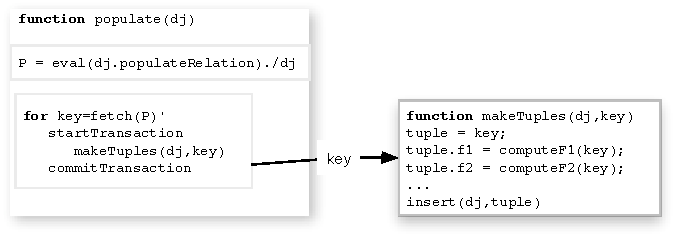
\includegraphics[width=0.85\textwidth]{populate.pdf}
\caption{Populating object \mcode{dj}.   }
\label{fig:populate}
\end{figure}


\subsection{Defining \mcode{makeTuples}}
The aim of the user-defined \mcode{makeTuples(dj,key)} callback is to create new tuples in relation \mcode{dj} for the given \mcode{key}. 

This function consists of the following sections:
\begin{enumerate}
\item fetch related data from parent tables or parents' parent tables for the given key.  

{\color{red}Important:} \mcode{makeTuples} should only retrieve data from tables that are direct ancestors of the present table or from their subtables. Fetching from tables that are not above the current table in the hierarchy may result in outdated tuples when the referenced data are changed. If data are needed from other tables, the schema should be updated to place the desired data above the current table.  This constraint is not currently enforced by DataJoint for the sake of performance. 
\item compute new values and from new tuples
\item insert the new tuples into the table
\end{enumerate}

\mcode{DeclareDJ} will automatically create a template with these section.  The example below is for the \mcode{CellTraces} class, which produces filtered versions of calcium traces:
\begin{lstlisting}
% CellTraces/makeTuples(this,key) - makes CellTraces tuples for the given key
function makeTuples(this,key)   

% get related data from parent tables
[cellnums,traces] = fetchn(Cells(key),'cellnum','calcium_trace');
fps = fetch1(ScansCorrected(key),'fps');

% filter traces
traces = [traces{:}];  % traces are in columns
traces = filterTraces(traces,fps,fetch(TraceOpts(key),'*'));

% insert cell traces one-by-one
for icell=1:length(cellnums)
    tuple = key;
    tuple.cellnum = cellnums(icell);
    tuple.trace = single(traces(:,icell));
    tuple.skewness = skewness( tuple.trace );
    
    insert( this, tuple );  % insert into table
end
\end{lstlisting}



\subsection{Populate Transactions}
Note that calls to \mcode{makeTuples} are performed within an atomic transaction (\autoref{fig:populate}): meaning that inserted tuples do not become visible to the rest of the world until the entire transaction is complete and that changes made by other processes do not become visible to \mcode{makeTuples} while it is executing.  If \mcode{makeTuples} fails to complete, any inserts that it has already done (including subtables) are rolled back and never become visible to other processes.  This feature makes DataJoint transaction-safe: interrupted processes do not leave incomplete data and processes running in parallel never see each other's incomplete data.


\section{Distributed Jobs}
\subsection{Defining the job method}
\subsection{Executing \mcode{runJob}}



\section{Appendix A: The Vis2p Schema}\label{sec:vis2p}
\subsection{Scenario}
The schema below represents the following simplified scenario: Our lab records neural activity data from mice. A recording session may include two-photon microscopy recordings with a variety of structural dyes and Ca$^{2+}$-sensitive dyes, optical imaging using intrinsic signals while the mouse views visual stimuli.  The processing chain extracts the neural signals from the raw recordings and computes several attributes of neural activity such as orientation tuning. 

\subsection{Entity relationship diagram}
The entity relationship diagram in \autoref{fig:erd} depicts the parent/child relationships between tables used in examples throughout this tutorial. To produce similar diagrams for your schemas, use the \mcode{erd} method.

\begin{lstlisting}
>> erd(Mice,false,'./core','./visual_stimuli');
\end{lstlisting}
\begin{figure}[h]
\center 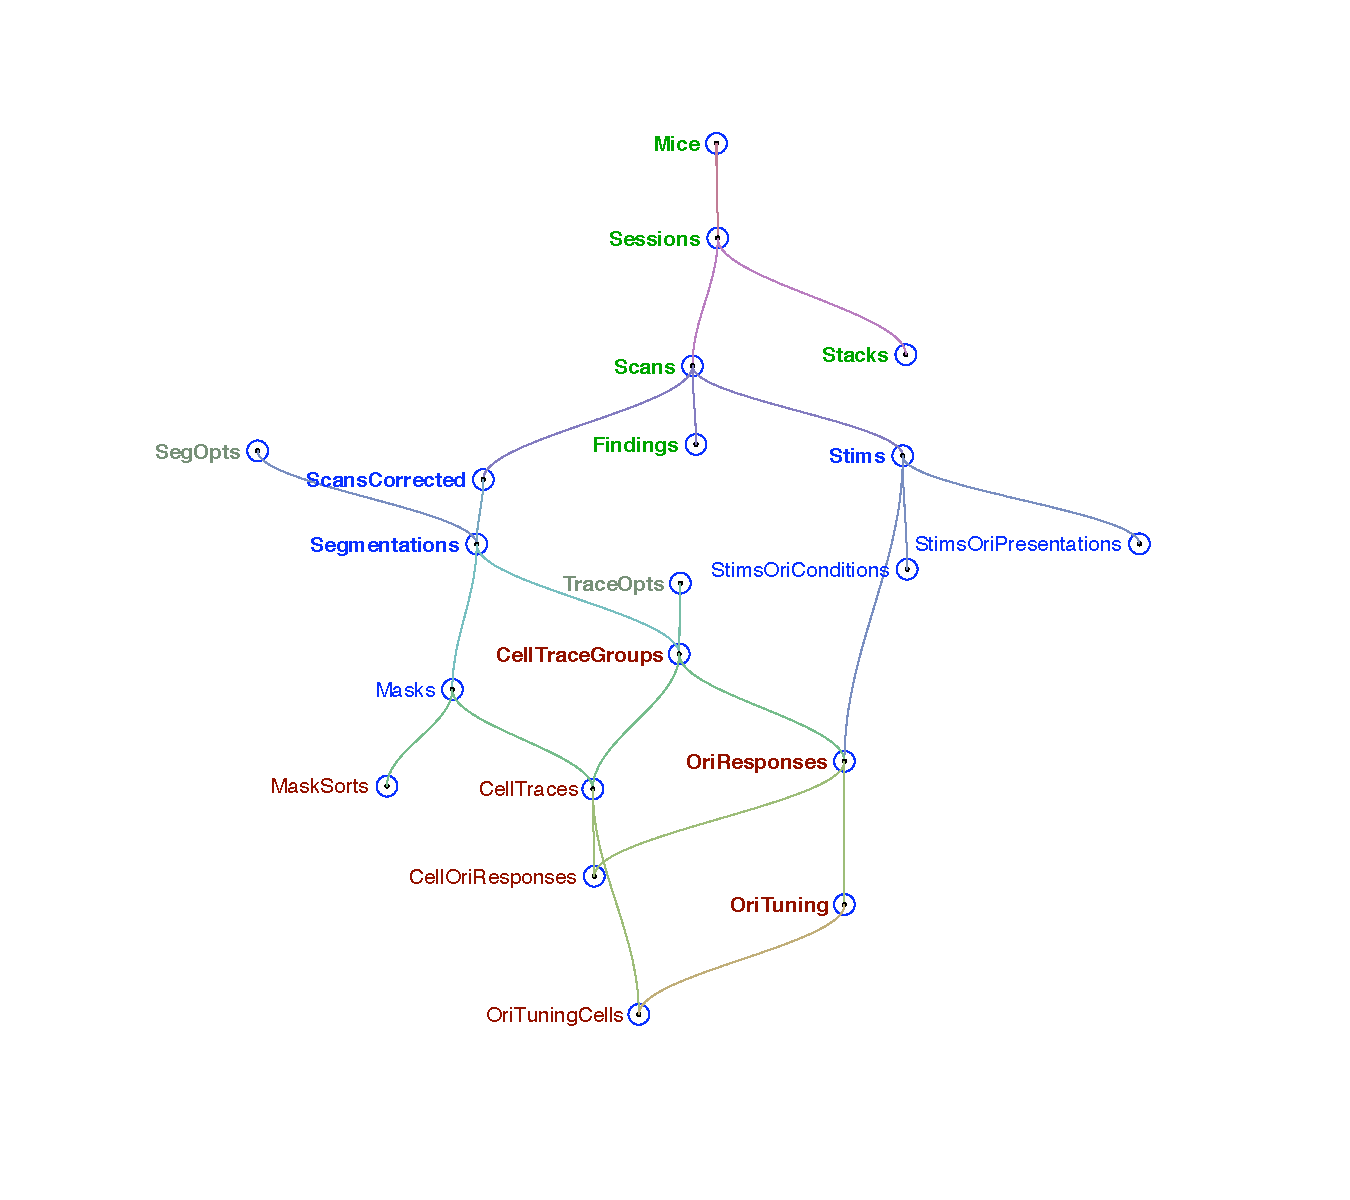
\includegraphics[width=0.9\textwidth]{erd.pdf}
\caption{The entity relationship diagram for the vis2p schema used in examples in this tutorial.  All dependencies are directed downward from a root table to dependent tables. Lookup tables are marked in gray, manual tables in green, imported in blue, and computed in red. Subtables (\autoref{sec:subtables}) are indicated in light font while all other tables are in bold.}
\label{fig:erd}
\end{figure}


\subsection{Declarations for Mice, Sessions, and Scans}
\begin{lstlisting}
%% Mice 
ddj=DeclareDJ( Vis2p, 'Mice','manual' );
ddj=addKeyField(ddj,'mouse_id','smallint unsigned','unique mouse id (0-65535)');

ddj=addField(ddj,'mouse_strain','enum("C57BL6/J","agouti")','');
ddj=addField(ddj,'mouse_dob','date','mouse date of birth');
ddj=addField(ddj,'mouse_sex','enum("F","M","unknown")','');
ddj=addField(ddj,'mouse_notes','varchar(1023)','free-text info about the mouse','');

ddj=execute(ddj);
setTableComment(Mice,'Information about mice');


%% Sessions
dj=DeclareDJ(Vis2p,'Sessions','manual');
ddj=addParent(ddj,Mice);
ddj=addKeyField(ddj,'sessnum','tinyint unsigned','imaging session number for this mouse');
ddj=addField(ddj,'sess_date','date','recording session date');
ddj=addField(ddj,'operator','enum("Dimitri","Manolis","Jacob")', 'experimenter"s name');
ddj=addField(ddj,'anesthesia','enum("none","urethane","isoflurane","fentanyl")',...
   'anesthesia type per protocol');
ddj=addField(ddj,'dye',...
   'enum("none","OGB","OGB+SR101","OGB+Alexa","GCaMP3","OGB+SR101+calcein")', ...
   'fluorescent dye combination');
ddj=addField(ddj,'directory','varchar(512)', ...
   'the present location of the 2-photon data and other recordings');
ddj=addField(ddj,'sess_notes','varchar(1023)','free-form notes about the imaging session','');

dj=execute(ddj);
setTableComment(Sessions,'Recording sessions');


%% Scans
ddj=DeclareDJ(Vis2p,'Scans','manual');
ddj=addParent(ddj,Sessions);
ddj=addKeyField(ddj,'scannum','smallint unsigned','scan number within the session');

ddj=addField(ddj,'lens','tinyint unsigned','lens magnification');
ddj=addField(ddj,'mag','decimal(4,2) unsigned','scan magnification');
ddj=addField(ddj,'laser_wavelength','smallint unsigned','(nm)');
ddj=addField(ddj,'laser_power','smallint unsigned','mW to prep');
ddj=addField(ddj,'x','int','(um) objective manipulator x position (assumed same reference thru session)',[]);
ddj=addField(ddj,'y','int','(um) objective manipulator y position (assumed same reference thru session)',[]);
ddj=addField(ddj,'z','int','(um) objective manipulator z position (assumed same reference thru session)',[]);
ddj=addField(ddj,'surfz','int','(um) objective manipulator z position at pial surface',[]);
ddj=addField(ddj,'scan_notes','varchar(256)','optional free-form comments','');

dj=execute(ddj);
setTableComment(Scans,'Two-photon movie scans but not stacks');
\end{lstlisting}

\subsection{Visual stimuli}\label{sec:visstims}
\begin{lstlisting}
%% Stims
ddj=DeclareDJ(Vis2p,'Stims','imported');
ddj=addParent(ddj,Scans);
ddj=setPopulateRelation(ddj,Scans);

dj=execute(ddj);
setTableComment(Stims,'Visual stimuli and two-photon synchronization');


%% StimsOriConditions
ddj=DeclareDJ(Vis2p,'StimsOriConditions','imported');
ddj=addParent(ddj,Stims);
ddj=addKeyField(ddj,'cond_idx','smallint unsigned','the condition index');

ddj=addField(ddj,'direction','decimal(4,1) unsigned','degrees, grating direction. 0=up, the clockwise');
ddj=addField(ddj,'contrast','decimal(4,3)','grating contrast');
ddj=addField(ddj,'luminance','float','grating luminance');
ddj=addField(ddj,'spatial_freq','float','(cycles/degree) grating spatial frequency');
ddj=addField(ddj,'temp_freq','float','(Hz) grating temporal frequency');
ddj=omitTimestamp(ddj);

dj=execute(ddj);
setTableComment(StimsOriConditions,'');


%% StimsOriPresentations
ddj=DeclareDJ(Vis2p,'StimsOriPresentations','imported');
ddj=addParent(ddj,Stims);
ddj=addKeyField(ddj,'presnum','smallint unsigned','presentation number');

ddj=addReference(ddj,StimsOriConditions);
ddj=addField(ddj,'onset','double','(ms) onset time relative to the first frame timestamp');
ddj=addField(ddj,'duration','smallint unsigned','(ms) duration of the condition presentation');

dj=execute(ddj);
setTableComment(StimsOriPresentations,'');
\end{lstlisting}

\section{Appendix B: Helpful SQL expression syntax}\label{sec:sql}
Conditions used in the restrict operator (\autoref{sec:restrict}) are specified in SQL syntax. Users need to know only a few SQL operators and functions to take full advantage of the restrict operator.  For additional information, consult the MySQL documentation available online. 
\subsection{comparison operators}
The comparison operators {\tt =}, {\tt <>}, {\tt >}, {\tt <}, {\tt >=}, and {\tt <=} are applicable to numbers, dates, timestamps, and strings. 
\begin{lstlisting}
Sessions('sess_date>"2011-03-01"')  % all sessions recorded after March 1, 2011
\end{lstlisting}
\subsection{logical operators}
The logical operators {\tt or}, {\tt and}, and {\tt not} are applied to results of boolean expressions.
\begin{lstlisting}
Scans('lens>10 and mag>1.5')  % all scans performed using objective lenses >x10 and scan magnification >1.5
\end{lstlisting}

\subsection{detecting missing values}
To detect missing values, one can use the operators {\tt is null} and {\tt is not null}:
\begin{lstlisting}
ScansDetected('raster_correction is not null'); % select scans in which raster correction was performed
\end{lstlisting}

\subsection{arithmetic operators and functions}
The arithmetic operators {\tt +}, {\tt -} (unitary and binary), {\tt *}, {\tt /}, {\tt \%} (modulo), and {\tt div} (integer division) are applicable to results of numerical expressions. 

In addition, mathematical functions can be applied to results of numeric expressions and their full list may be found at 
\url{http://dev.mysql.com/doc/refman/5.5/en/mathematical-functions.html}.

\subsection{membership operators}
The membership operators {\tt in} and {\tt not in} can simplify comparisons to a set of values: 
\begin{lstlisting}
% get all sessions with urethane and isoflurane anesthesia performed by anyone other than Dimitri or Manolis
Sessions('operator not in ("Dimitri","Manolis") and anesthesia in ("urethane","isoflurane")')
\end{lstlisting}

\subsection{date and time functions}
The full list of date and time functions may be found at \url{http://dev.mysql.com/doc/refman/5.5/en/date-and-time-functions.html}.  
\begin{lstlisting}
restrict(Sessions*Mice,'datediff(sess_date,mouse_dob)>=21') % all sessions performed on mice 21 days and older
\end{lstlisting}

\subsection{aggregate functions}
Aggregate functions can only be used to define new fields using the summarize operator (\autoref{sec:summarize}).  They are described in detail at \url{http://dev.mysql.com/doc/refman/5.5/en/group-by-functions.html}.

\section{Appendix C: Internal conventions}
DataJoint uses a number of internal conventions and constraints. These do not need to be understood in normal use.

\subsection{Table names}
Table names are converted from the CamelCase names of their classes to underscore-delimited compound names with an underscore preceding every capital letter.

Lookup table names are prefixed with the pound sign \#; imported tables are preceded with a single underscore \_; and computed tables are preceded with a double underscore \_\_. 

For example, the database name for the lookup table \mcode{TraceOpts} is {\tt \#trace\_opts}, manual table \mcode{Scans} becomes {\tt scans}, and computed table \mcode{TraceQuality} is {\tt \_\_trace\_quality}.

\subsection{Foreign keys}

\end{document}